\chapter{場景設計}
\section{設計理念}
 當初會想到這樣畫是因為想要更接近實際的樣貌,所以才會多做一個觀眾席和路燈。想讓這個遊戲玩起來更真實,更貼近生活。\\[6pt]
\begin{figure}[hbt!]
\begin{center}
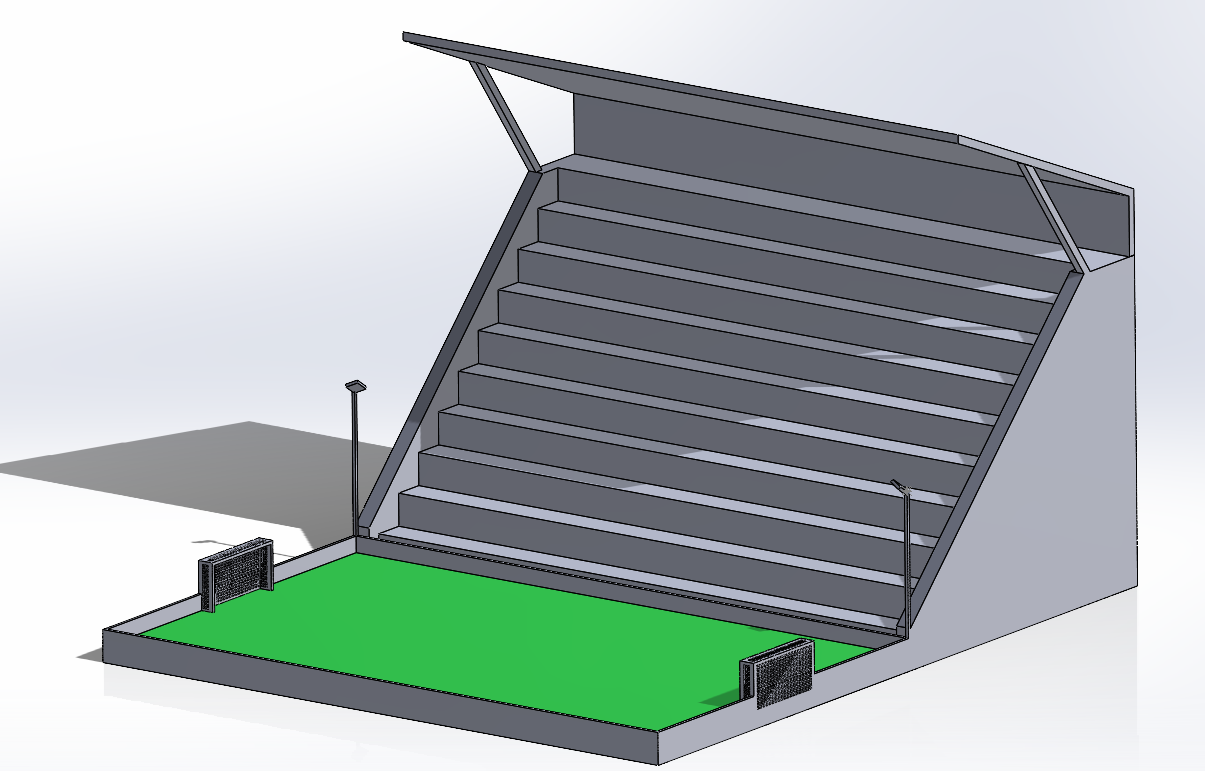
\includegraphics[height=6cm]{場景}
\caption{\Large 場景}\label{場景}
\end{center}
\end{figure} 

\newpage

\section{設計更改}

將原本的場景放入CopppeliaSim時,因為球門的網格太細而出現模型計算的問題,導致在執行程式或操控球員時,會發生很嚴重的延遲。修改過後將球門設為平滑面,再執行一次就沒有模型計算問題了。\\[6pt]

\begin{figure}[hbt!]
\begin{center}
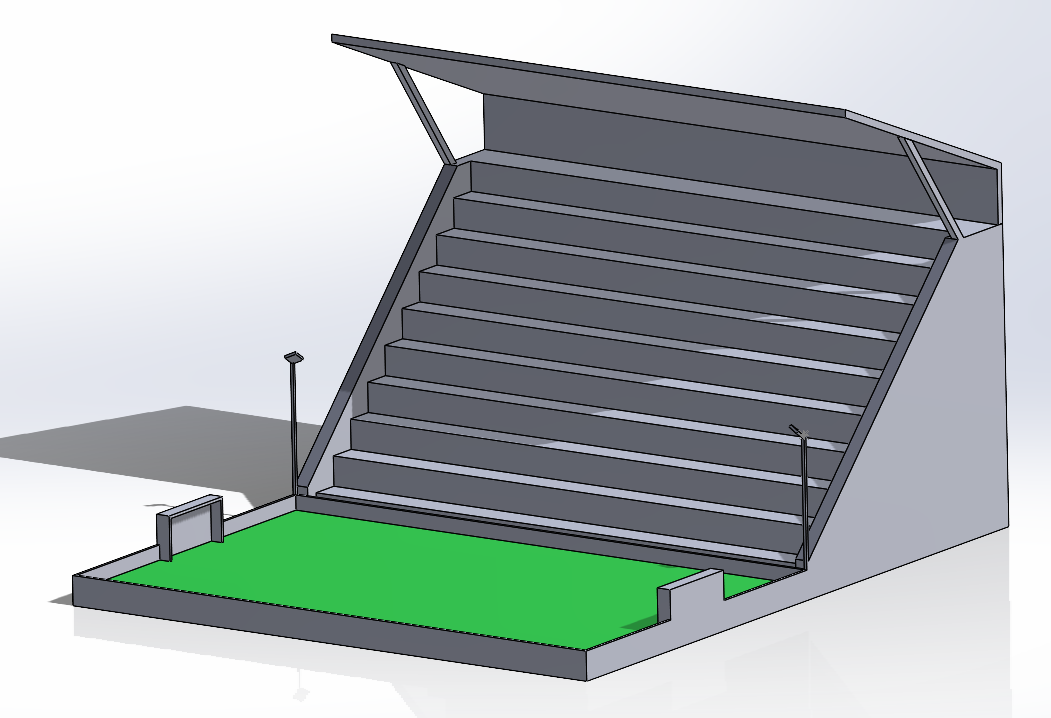
\includegraphics[height=6cm]{場景new}
\caption{\Large 修改後場景}\label{場景new}
\end{center}
\end{figure} 

\newpage